\chapter{Additional figures}\label{apx:additiona-figures}
\begin{figure}[!htbp]
  \centering
  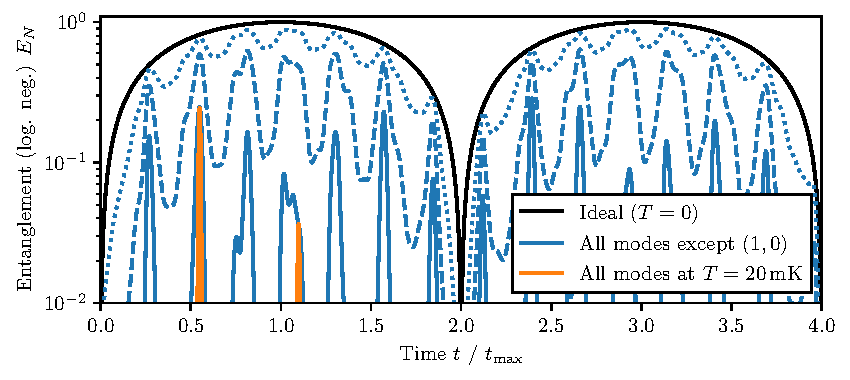
\includegraphics[width=\textwidth]{./../figures/vibrations/entanglement-dynamics-all-modes_rs-5mm.pdf}
  \caption{Similar to \cref{fig:5:entanglement-multiple-modes} at $T=20\si{mK}$ for a smaller shied with $r_s = 5\si{mm}$ at a separation of $L=2R = 20\si{\mu m}$, where the particle is placed at the worst-case position in front of the shield, where the effects of the mode $(1,0)$ are maximized.}
  \label{fig:apx:entanglement-thermal-shield-rs-5mm}
\end{figure}

\begin{figure}[!htbp]
  \centering
  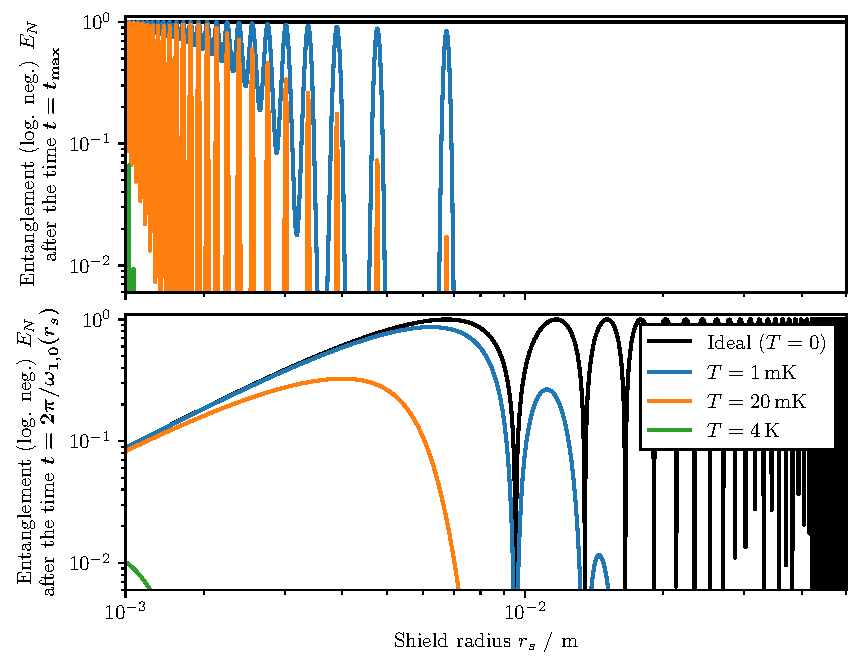
\includegraphics[width=\textwidth]{./../figures/vibrations/all-modes-entanglement-rs.pdf}
  \caption{Generated entanglement after \textbf{(top)} a time $t_\mathrm{max} = 259\si{ms}$ and after \textbf{(bottom)} a time $2\pi/\omega_{1,0}(r_s)$ for different shield radii $r_s$. The plotted concept is similar to \cref{fig:5:entanglement-thermal-shield-L}. A smaller shield Parameters from \cref{tab:paramters} were taken. The artifacts at around $r_s \approx 5\times 10^{-2}\si{m}$ in the bottom figure are due to numeric instabilities.}
  \label{fig:apx:entanglement-thermal-shield-rs}
\end{figure}